\chapter{Experimentation, Results and Discussion}
\label{ch:results}

This chapter first revisits the Phase 2 results, because two of them did not survive Phase 3. It then
reports the training diagnostics, the identity factors, the image-blind constant, and the answers to
RQ1--RQ3. It ends with the abnormality flag, the controls, runtime, a discussion and the limitations.
Unless stated otherwise, intervals are 95\% paired cluster-bootstrap intervals over images, and
differences are system minus comparator in percentage points. % {C095}

\section{Phase 2 Results Revisited}
\label{sec:res-phase2}

The Phase 2 report presented the results in Table~\ref{tab:p2results} and
Figures~\ref{fig:p2train}--\ref{fig:p2cejagree}. They are kept here as they were measured, and
Table~\ref{tab:p2corrections} states what Phase 3 found about each.

\begin{table}[!htbp]
\centering
\caption[Phase 2 results as reported]{Phase 2 results as reported (Phase 2 report, Tables 6.1 and
6.2), all on validation splits.}
\label{tab:p2results}
\small
\begin{tabularx}{\textwidth}{@{}L{4.0cm}YYL{3.6cm}@{}}
\toprule
Module & Headline & Other figures & Evaluation set\\
\midrule
Bone-loss binary & macro-F1 0.9233 & sensitivity 0.8305, specificity 0.9953 & 1,558 validation crops\\
Bone-loss severity & macro-F1 0.7208 & mild-class F1 0.80 & positive subset (mild $n = 6$)\\
Caries severity (final cascade run) & macro-F1 0.77 & accuracy 0.81, deep-caries recall 0.84 & 133 validation crops\\
CEJ heuristic & reliable on 62.5\% & exact agreement 15.1\%, within one class 61.6\% & 296 crops\\
\bottomrule
\end{tabularx}
\end{table}

\begin{figure}[!htbp]
\centering
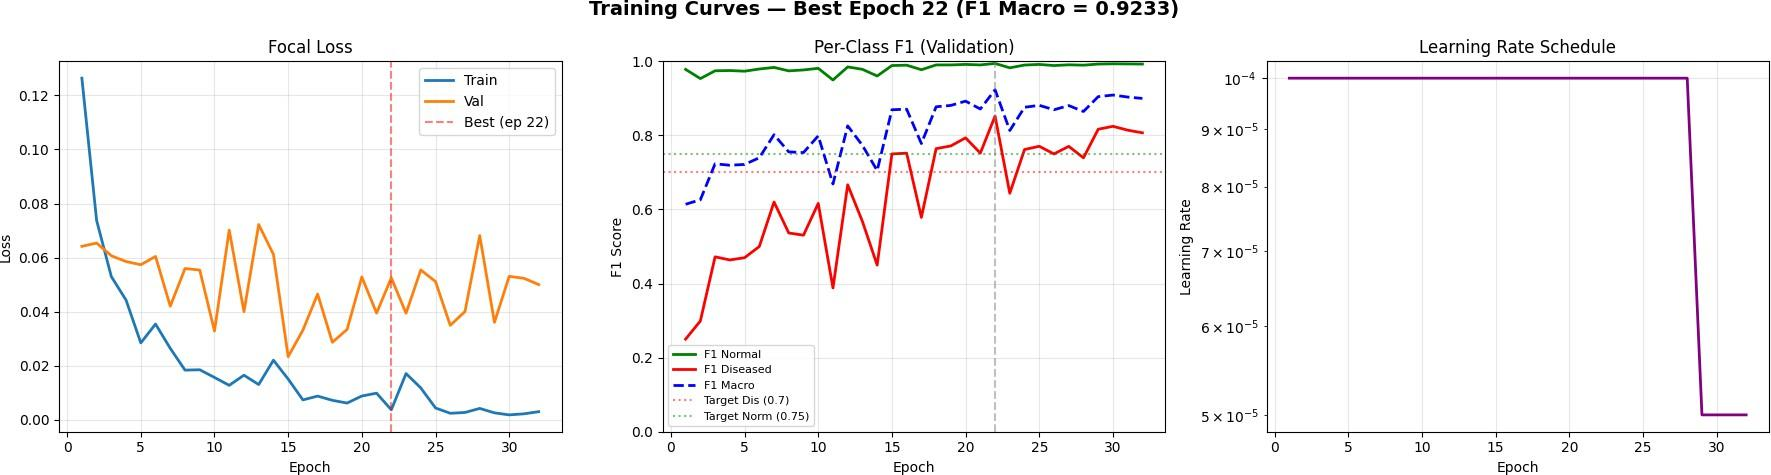
\includegraphics[width=0.92\textwidth]{figures/phase2/p2_6_01_boneloss_training.jpg}
\caption[Phase 2 training curves of the binary bone-loss classifier]{Training and validation curves of
the Phase 2 binary bone-loss classifier (Phase 2 report, Figure 6.1). Its validation split shared
radiographs with training; see Table~\ref{tab:p2corrections}.}
\label{fig:p2train}
\end{figure}

\begin{figure}[!htbp]
\centering
\begin{subfigure}[b]{0.56\textwidth}
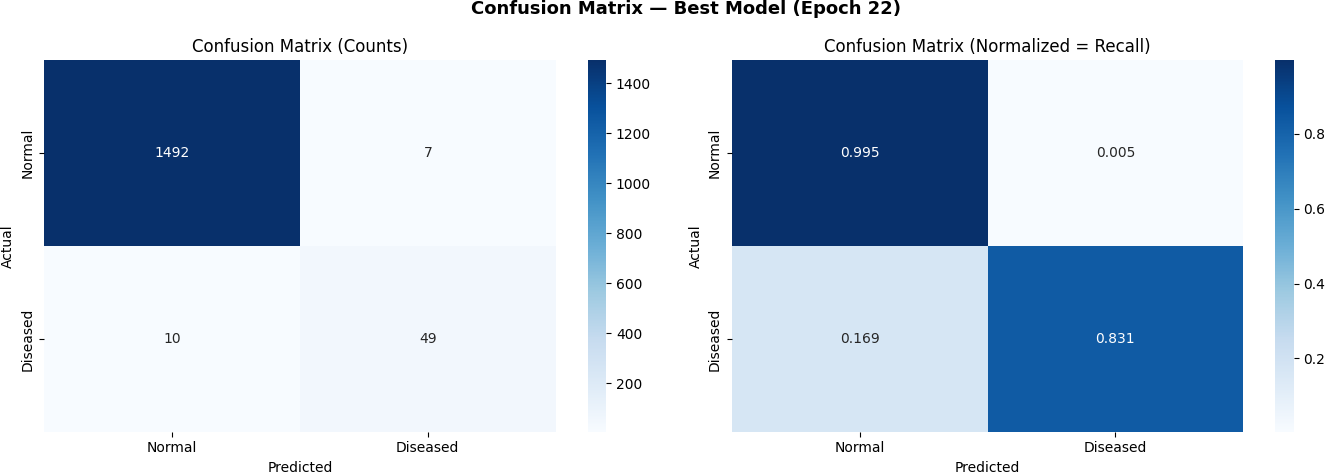
\includegraphics[width=\textwidth]{figures/phase2/p2_6_02_boneloss_confusion.png}
\caption{Binary model, validation split.}
\label{fig:p2cm}
\end{subfigure}\hfill
\begin{subfigure}[b]{0.42\textwidth}
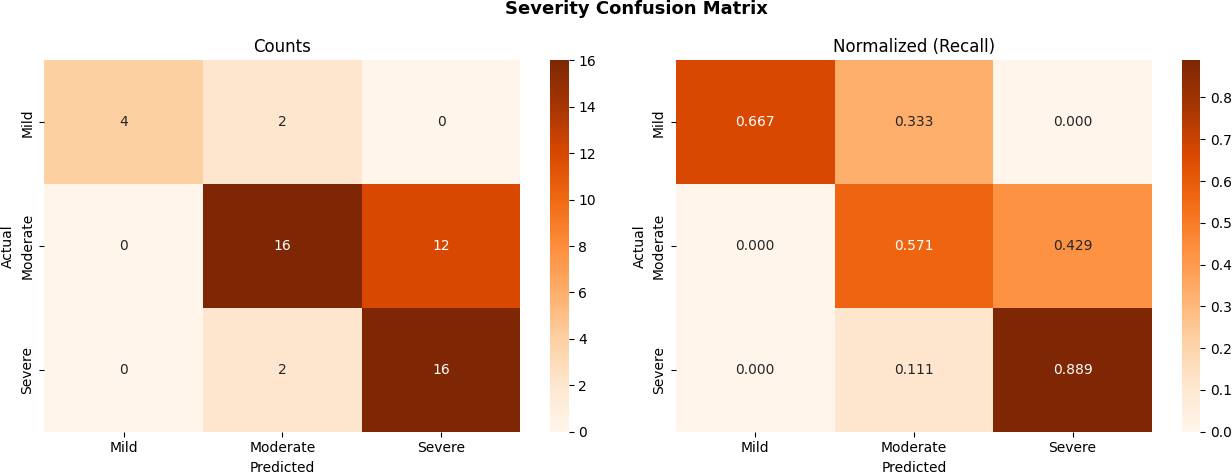
\includegraphics[width=\textwidth]{figures/phase2/p2_6_03_severity_confusion.png}
\caption{Severity model, positive subset.}
\label{fig:p2sev}
\end{subfigure}
\caption[Phase 2 confusion matrices]{Phase 2 confusion matrices (Phase 2 report, Figures 6.2 and
6.3).}
\label{fig:p2confusions}
\end{figure}

\begin{figure}[!htbp]
\centering
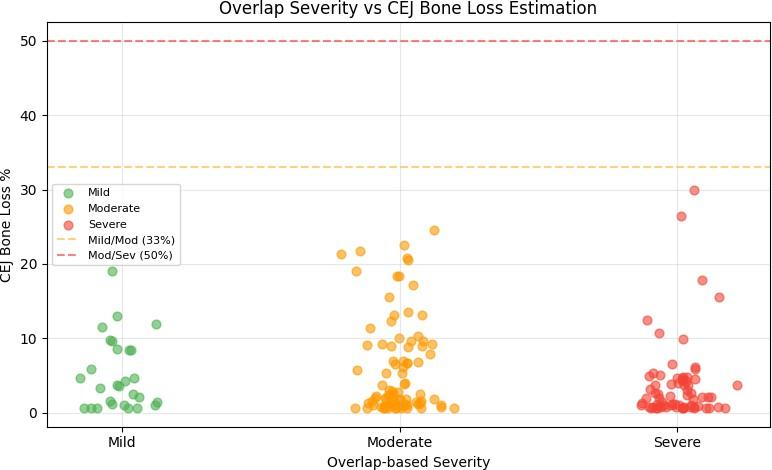
\includegraphics[width=0.62\textwidth]{figures/phase2/p2_6_04_cej_vs_overlap.jpg}
\caption[Phase 2 CEJ estimation against overlap severity]{Agreement of the CEJ heuristic with the
overlap-based severity labels (Phase 2 report, Figure 6.4).}
\label{fig:p2cejagree}
\end{figure}

\begin{table}[!htbp]
\centering
\caption[What Phase 3 found about the Phase 2 results]{What Phase 3 found about each Phase 2 result.}
\label{tab:p2corrections}
\small
\begin{tabularx}{\textwidth}{@{}L{3.6cm}Y@{}}
\toprule
Phase 2 result & Phase 3 finding\\
\midrule
Bone-loss binary, macro-F1 0.9233 & A crop-level split: every validation radiograph also supplied training crops. Held out by radiograph, the same model finds 3.4\% of labelled teeth (6 of 175); retrained by radiograph, 27.5\% at 95.9\% specificity (Section~\ref{sec:res-stage4})\\
``Bone loss'' label & The masks mark apical lesions, sclerosis and cysts; the output is reported as an abnormality flag\\
Bone-loss severity, macro-F1 0.7208 & Classes came from crop contrast; retrained on true overlap bands, 0.294 against 0.334 for a tooth-position prior: withheld\\
Caries severity, macro-F1 0.77 & Kept as Stage 3b; validated on the same 133 crops, not evaluated separately here\\
CEJ heuristic & Unchanged: a documented negative result\\
Integration ``not yet implemented'' & Six stages run end to end (Chapters~\ref{ch:system} and~\ref{ch:impl})\\
\bottomrule
\end{tabularx}
\end{table}
% {C040} {C041} {C042}

\section{Training Diagnostics}
\label{sec:res-train}

Every training loss in Figure~\ref{fig:training} falls steadily. Each kept checkpoint is the best on
its run's validation split, so these are selection diagnostics, not test results. % {C032}
\begin{itemize}
\item \textbf{Tooth detector.} Validation box mean average precision at IoU 0.5 (mAP@0.5) reaches
  0.634 at its last epoch and is still rising. On the frozen Tufts test split it missed its
  pre-registered guard, which required it to stay within four points of a Tufts-only control
  (0.587 against 0.723). It was adopted regardless, by a dated decision, for its numbering and caries
  behaviour.
\item \textbf{Lesion detector.} It peaks at mAP@0.5 0.820 (epoch 29 of 54).
\item \textbf{Numbering head.} Crop-level FDI-exact accuracy reaches 0.810 (epoch 12 of 15). The
  quadrant digit is right on 98.1\% of crops and the position digit on 82.5\%, so its errors are
  counting errors along the arch.
\item \textbf{Stage 4a.} Validation macro-F1 stays below 0.6 in all three seeds (best 0.568, 0.580
  and 0.597).
\end{itemize}
% {C031} {C032}

\begin{figure}[!htbp]
\centering
\includegraphics[width=\textwidth]{figures/repo/R04_training.pdf}
\caption[Training logs of the four trained stages]{Training logs of the four trained stages, from the
saved run files; validation splits, not test. (a) Tooth detector, 148 epochs, 150 Tufts radiographs.
(b) Lesion detector, 54 epochs, 1,200 CariesXrays radiographs. (c) Numbering head, 15 epochs, 6,450
tooth crops (DENTEX and Tufts, ground-truth boxes). (d) Stage-4a flag, three seeds of one recipe.
Dots: the checkpoint each run kept.}
\label{fig:training}
\end{figure}

On a published benchmark the detector family is competitive. Trained on CariesXrays alone, the lesion
detector's single-corpus arm reaches COCO AP 48.2 (AP50 84.5) on the project's seed-fixed 1,200-image
validation split. That matches the benchmark authors' task-specific method (48.2, AP50 84.1) and is six
points above the strongest of their ten baselines (42.2)~\cite{chen2024cariesxrays}. The splits
differ, and the project's split also chose the checkpoint, so the comparison is indicative only;
Section~\ref{sec:res-rq2} shows that this checkpoint does not transfer. The earlier detector lever is
summarised in Figure~\ref{fig:lever1}. % {C033}

\begin{figure}[!htbp]
\centering
\includegraphics[width=0.86\textwidth]{figures/repo/lever1_summary.png}
\caption[Lever 1, the first multi-corpus detector]{Lever 1, the first multi-corpus detector: numbering
on 164 DENTEX images rose (left), but the Tufts box-mAP guard failed (right), so it stayed an ablation.
Its successor, Lever A, is the shipped detector.}
\label{fig:lever1}
\end{figure}

\section{Identity: Detection and Numbering}
\label{sec:res-identity}

Table~\ref{tab:identity} measures the first two factors of the decision chain~\eqref{eq:chain}. On
DENTEX, whose other images trained the detector, identity costs 7.2 points. On the Tufts test split,
also from a training corpus, it costs 36.5. On UFBA-425, which no model trained on, it costs 55.5
points with the files as distributed. % {C030}

\begin{table}[!htbp]
\centering
\caption[Identity before disease]{Identity before disease: the first two factors of~\eqref{eq:chain},
per tooth, in percent. Det.: detected; Exact: numbered exactly, of those detected; End to end: their
product, with a 95\% cluster-bootstrap interval. DENTEX 164 images, Tufts test 143, UFBA-425 425 (as
distributed, and widened to a panoramic shape).}
\label{tab:identity}
\small
\begin{tabular}{@{}lrrrr@{}}
\toprule
Corpus & Teeth & Det. & Exact & End to end\\
\midrule
DENTEX & 936 & 99.6 & 93.2 & 92.8 [90.6, 94.9]\\
Tufts test & 3,760 & 89.3 & 71.1 & 63.5 [59.3, 67.5]\\
UFBA as is & 11,591 & 66.6 & 66.8 & 44.5 [42.4, 46.6]\\
UFBA widened & 11,591 & 95.6 & 80.8 & 77.2 [75.2, 79.1]\\
\bottomrule
\end{tabular}
\end{table}

End-to-end FDI-exact accuracy on DENTEX is 92.8\% (869 of 936 teeth) [90.6, 94.9], an in-domain
figure. Four teeth are not detected, and 93.2\% of the 932 found are numbered correctly. Of 63 wrong
codes, 51 (81.0\%) name an adjacent tooth in the correct quadrant (29 one step towards the midline, 22
one step away), and only 6 of 932 detected teeth (0.6\%) receive a quadrant-level error
(Figures~\ref{fig:numbering} and~\ref{fig:taxonomyerr}). Errors concentrate where adjacent teeth look
alike: 11.3\% of detected lateral incisors and 10.1\% of central incisors receive a wrong code,
against 4.1\% of second premolars. At molar positions, where most caries lies, 8.2\% of detected
second molars receive a wrong code, and each such error moves any finding to the wrong tooth. % {C034}

\begin{figure}[!htbp]
\centering
\includegraphics[width=\textwidth]{figures/repo/R08_numbering_reliability.pdf}
\caption[Outputs a constant cannot produce]{Outputs a constant cannot produce. (a) Numbering outcome
for each of 936 ground-truth DENTEX teeth (log scale). (b) Share of detected teeth given a wrong code,
by position. (c) Accuracy on the items answered as the least confident are declined: numbering, from
saved per-tooth confidences (circle: the 0.30 threshold fixed in code); crop classifier, saved
operating points at 50, 75, 90 and 100\% coverage. (d) Reliability of the crop classifier's raw
confidence on 863 held-out crops, by stated probability (marker area proportional to bin count).}
\label{fig:numbering}
\end{figure}

\begin{figure}[!htbp]
\centering
\includegraphics[width=0.94\textwidth]{figures/repo/stage2_failure_taxonomy_arm3c.png}
\caption[Numbering outcome taxonomy under the shipped detector]{Numbering outcome taxonomy under the
shipped detector, 936 DENTEX teeth: outcome categories (left) and the error rate by tooth position
(right).}
\label{fig:taxonomyerr}
\end{figure}

\section{The Positional Prior and the Image-Blind Constant}
\label{sec:res-constant}

On the fit set (Figure~\ref{fig:prior}) rule~\eqref{eq:rule} admits the eight first and second molars,
with prevalences from 0.372 (tooth 26) to 0.205 (tooth 27). It rejects the ninth code, tooth 15, at
0.128 against a threshold of 0.196, which is exactly the set the evaluation's greedy search returns.
Frozen, \{16, 17, 26, 27, 36, 37, 46, 47\} scores F1 0.392 on its fit images and 0.320 on the 164
scored ones: 286 true positives among 1,312 named codes, against 477 carious teeth, so its recall is
0.600, the share of carious teeth that lie on those eight molars. The prior shifts between the two
sets: teeth 17 and 27 fall to 0.140 and 0.134 on the scored images, so the oracle constant fitted on
the scored images themselves keeps six molars and reaches only 0.330. Almost all of the image-blind
score therefore needs no evaluation data. % {C010} {C011}

The set is fragile at its margin and the floor is not (Figure~\ref{fig:stability}). Refitted on 10,000
resamples of the fit images, rule~\eqref{eq:rule} returns exactly these eight molars 27\% of the time
and seven codes 45\% of the time, yet the refitted constants score a median F1 of 0.320 on the scored
images, 95\% of them between 0.279 and 0.330. Over sizes one to sixteen the constant's F1 is flat from
six to nine codes (0.298 to 0.325; Figure~\ref{fig:opcurve}). % {C012}

\begin{figure}[!htbp]
\centering
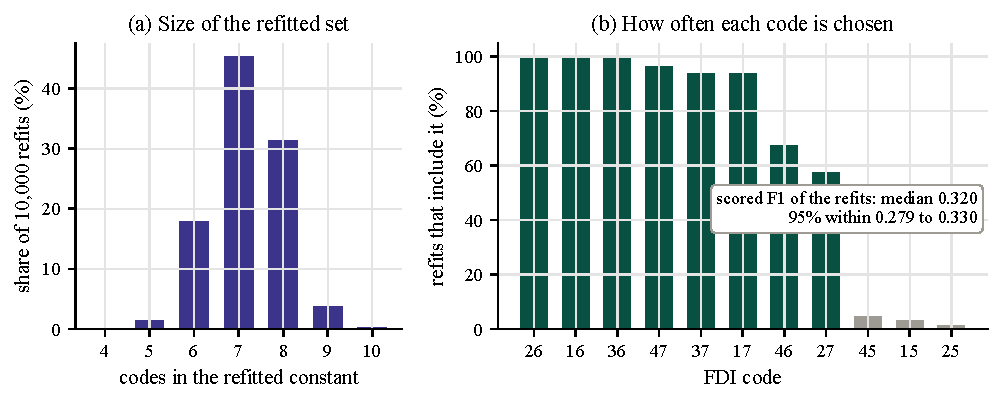
\includegraphics[width=\textwidth]{figures/plots/P2_constant_stability.pdf}
\caption[Stability of the fitted constant]{Stability of the fitted constant over 10,000 resamples of
the 78 fit images. (a) Size of the refitted set. (b) How often each code is chosen (teal: the eight
molars).}
\label{fig:stability}
\end{figure}

\begin{figure}[!htbp]
\centering
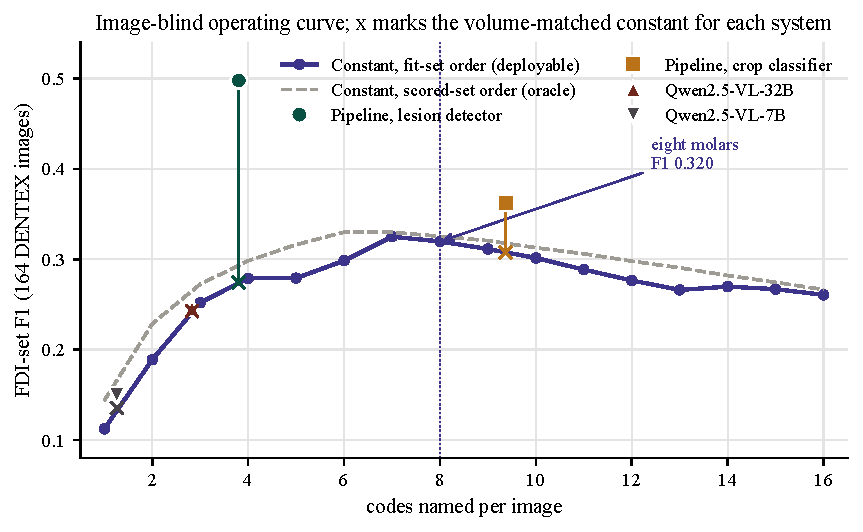
\includegraphics[width=0.94\textwidth]{figures/plots/P1_operating_curve.pdf}
\caption[Image-blind operating curve]{Image-blind operating curve: F1 of the $k$ most prevalent codes,
in fit-set order (deployable) and scored-set order (oracle), with each system at its own output volume.
A cross marks the image-blind answer that names as many codes as the system.}
\label{fig:opcurve}
\end{figure}

\section{RQ1 on Development Data}
\label{sec:res-rq1dev}

\begin{table}[!htbp]
\centering
\caption[Tooth-level caries prediction on DENTEX]{Tooth-level caries prediction on 164 DENTEX images
(477 carious teeth), micro-averaged. P: precision; R: recall; Matched: F1 minus that of a constant
naming as many codes (pp).}
\label{tab:ladder}
\small
\begin{tabular}{@{}lrrrr@{}}
\toprule
System & P & R & F1 & Matched\\
\midrule
Pipeline, lesion detector & 0.439 & 0.574 & 0.498 & +22.35\\
Pipeline, crop classifier & 0.237 & 0.765 & 0.362 & +5.50\\
Constant (image-blind) & 0.218 & 0.600 & 0.320 & ---\\
Qwen2.5-VL-32B, zero-shot & 0.250 & 0.243 & 0.246 & +0.39\\
Qwen2.5-VL-7B, zero-shot & 0.248 & 0.107 & 0.149 & +1.39\\
Oracle constant (test-fitted) & 0.245 & 0.505 & 0.330 & ---\\
\bottomrule
\end{tabular}
\end{table}
% {C013} {C014}

Both vision-language models see the radiograph and score below a list that does not
(Table~\ref{tab:ladder}): $-7.32$ points [$-11.23$, $-3.42$] for the 32B model and $-17.04$ [$-21.22$,
$-12.66$] for the 7B. The crop-classifier pipeline leads the constant by $+4.27$ points [$+1.58$,
$+7.05$] while naming 1,537 teeth to its 1,312, at barely higher precision (0.237 against 0.218), as
expected of a classifier that leans on the prior. The lesion-detector pipeline leads by $+17.80$
[$+13.48$, $+22.02$] and is the only system whose precision clearly exceeds the constant's: it names
624 codes, 43.9\% of them carious. % {C013} {C014}

Volume explains neither pipeline lead (Figure~\ref{fig:matched}). Against a matched constant that
names as many codes as the system, the leads are $+5.50$ [$+2.84$, $+8.22$] for the crop classifier and
$+22.35$ [$+17.42$, $+27.18$] for the lesion detector. The vision-language models are level with
constants of their own volume (32B [$-4.90$, $+5.63$], 7B [$-2.06$, $+4.85$]): they fall below the
eight molars by naming fewer teeth, and their F1 carries no detectable image information. % {C015}

\begin{figure}[!htbp]
\centering
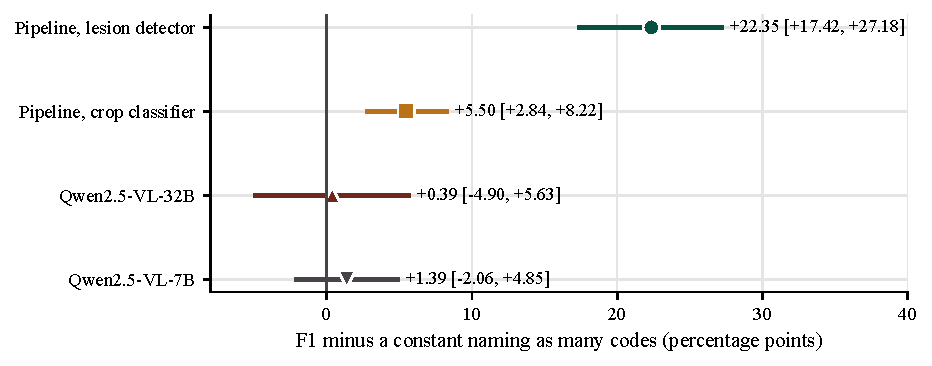
\includegraphics[width=0.86\textwidth]{figures/plots/P3_matched_volume.pdf}
\caption[Comparison at matched output volume]{Each system's F1 minus that of an image-blind answer
naming as many codes, with paired 95\% intervals over the 164 images.}
\label{fig:matched}
\end{figure}

Under lesion agreement the crop classifier leads the constant by $+17.12$ points [$+12.15$, $+21.89$],
partly by volume: it flags 1,439 teeth against 988, at a lower match rate (0.267 against 0.306). The
lesion detector flags 603 teeth at the highest match rate (0.473) and is not separable from the
constant ($-3.55$ [$-10.11$, $+2.64$]); F1 ranks it above the crop classifier, and agreement below.
None of this is yet evidence of perception, because the front end trained on this corpus. % {C025}

\section{RQ1 on External Data}
\label{sec:res-rq1ext}

On the four Ningxia sites the crop-classifier pipeline and the constant are level when pooled: 0.600
against 0.591, a difference of $+0.89$ points [$-3.86$, $+5.57$] (Figure~\ref{fig:paired}a). Per site,
the difference runs from $-18.99$ [$-26.32$, $-11.84$] at test1 to $+12.32$ [$+5.01$, $+19.20$] at test2
(Figure~\ref{fig:paired}b), a 31-point swing within one cohort. The constant's own agreement, each
site's prior mass on the eight molars, ranges from 0.494 to 0.709 (Figure~\ref{fig:sites}). On
CariesXrays the constant wins outright, 0.604 against 0.379 ($-22.42$ points [$-24.62$, $-20.18$]); it
flags 46\% more teeth but at the higher match rate (0.200 against 0.188), so volume does not explain it.
The crop-classifier pipeline leads only where its detector trained. % {C016}

\begin{figure}[!htbp]
\centering
\includegraphics[width=0.62\textwidth]{figures/repo/R07_paired_differences.pdf}
\caption[Lesion agreement of each caries option minus the constant]{Lesion agreement of each Stage-3a
option minus the constant, paired 95\% cluster-bootstrap intervals (10,000 resamples). (a) Per cohort;
DENTEX is development data for the front end and CariesXrays is the lesion detector's validation split.
(b) The four Ningxia sites, the pooled difference with sites fixed, and the DerSimonian--Laird mean for
the lesion detector (diamond; bar: 95\% interval; dotted, beyond the axis: prediction interval for a new
site).}
\label{fig:paired}
\end{figure}

\begin{figure}[!htbp]
\centering
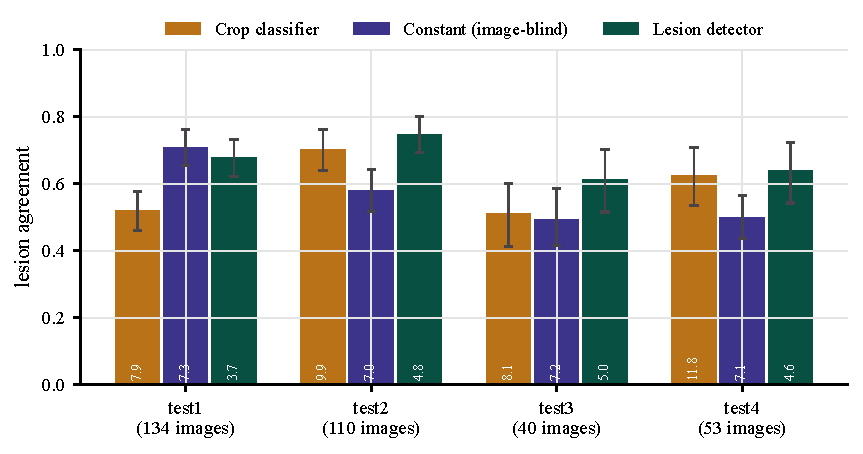
\includegraphics[width=0.92\textwidth]{figures/plots/P7_ningxia_sites.pdf}
\caption[Lesion agreement at each Ningxia site]{Lesion agreement at each Ningxia site for the three
Stage-3a options, with 95\% intervals. The numbers inside the bars are teeth flagged per image.}
\label{fig:sites}
\end{figure}

\section{RQ2: Localising Lesions Instead of Classifying Teeth}
\label{sec:res-rq2}

Five direct repairs of the crop classifier came first (Table~\ref{tab:repairs}), each against a same-day
control under a rule fixed in advance. None separated from zero, including a retrain with 2.67 times the
carious crops, so the ceiling is not set by supervision. Section~\ref{sec:res-shortcut} locates it in
the task as posed: a tight crop, a binary label and a strong prior. % {C017}

\begin{table}[!htbp]
\centering
\caption[Repairs of the crop classifier]{Repairs of the crop classifier on the same 863 held-out crops
(34 radiographs): paired difference in AP against the control (in F1 for the thresholds).}
\label{tab:repairs}
\small
\begin{tabular}{@{}lr@{}}
\toprule
Repair & Difference [95\% CI]\\
\midrule
Contrast equalisation (CLAHE) & $+0.049$ [$-0.003$, $+0.099$]\\
Crop expanded 1.25 times & $+0.020$ [$-0.037$, $+0.081$]\\
Position-balanced sampling & $+0.043$ [$-0.033$, $+0.116$]\\
Retrain, 2.67 times the positives & $-0.002$ [$-0.089$, $+0.082$]\\
Per-tooth-type thresholds (F1) & $+0.006$ [$-0.034$, $+0.041$]\\
\bottomrule
\end{tabular}
\end{table}

The task was then changed. Under the tooth detector of the time, the lesion detector met the
pre-registered rule on two cohorts of three: $+12.2$ points [$+10.1$, $+14.3$] over the constant on
CariesXrays and $+10.2$ [$+6.3$, $+14.0$] on Ningxia, with a tie on DENTEX ($-3.3$ [$-8.4$, $+1.3$]).
It was adopted on 4 September 2026. Table~\ref{tab:arms} gives the three options under the current
detector. % {C020} {C021}

\begin{table}[!htbp]
\centering
\caption[Lesion agreement of the three caries options]{Lesion agreement of the three Stage-3a options
under the current tooth detector: crop classifier (Clf.), constant (Const.) and lesion detector (Det.);
last column, detector minus constant in points, paired 95\% CI. CariesXrays is the detector's
validation split.}
\label{tab:arms}
\small
\begin{tabular}{@{}lrrrr@{}}
\toprule
Cohort & Clf. & Const. & Det. & Det.\ minus const.\\
\midrule
DENTEX & 0.802 & 0.630 & 0.595 & $-3.55$ [$-10.11$, $+2.64$]\\
CariesXrays & 0.379 & 0.604 & 0.757 & $+15.38$ [$+12.96$, $+17.73$]\\
Ningxia & 0.600 & 0.591 & 0.684 & $+9.28$ [$+4.72$, $+13.73$]\\
\bottomrule
\end{tabular}
\end{table}

Both consequences predicted in Section~\ref{sec:method-constant} hold.
\begin{itemize}
\item \textbf{Fewer flags.} The lesion detector flags 4.35 teeth per image against the constant's 7.15
  on Ningxia, and 2.16 against 7.05 on CariesXrays.
\item \textbf{More precise flags within each tooth type.} On DENTEX, the development corpus where
  per-type records exist, 46.3\% of the molars it flags carry caries, against 28.4\% for the crop
  classifier and 21.8\% for the constant; and 39.7\% of its flagged premolars against 17.0\%.
\end{itemize}
% {C023}
Per site (Figure~\ref{fig:pooling}) it is separated from the constant at test2, test3 and test4 ($+16.91$
[$+9.17$, $+24.62$], $+11.73$ [$+1.07$, $+21.34$], $+13.98$ [$+2.34$, $+24.34$]) and not at test1 ($-3.16$
[$-10.56$, $+3.97$]), where the constant is strongest. Treating the sites as a sample (random effects,
post hoc) gives $+9.61$ [$-0.54$, $+19.76$] (HKSJ [$-5.02$, $+24.24$]), $I^2 = 81\%$, $\tau$ 9.27 points
[3.22, 33.09] and a prediction interval of [$-36.08$, $+55.29$]. The lead therefore holds at three of
these four sites and is not shown for an unseen one. The training mixture, not the architecture,
transfers: the single-corpus arm reached 0.694 [0.674, 0.714] on CariesXrays but collapsed to 0.086
[0.055, 0.119] on DENTEX and 0.240 [0.209, 0.272] on Ningxia. % {C022} {C023} {C024}

\begin{figure}[!htbp]
\centering
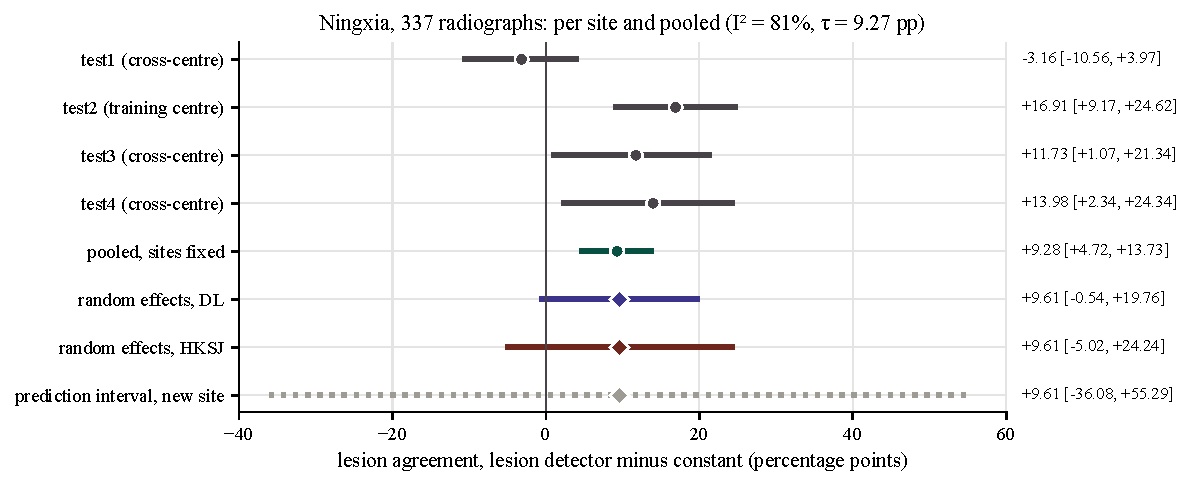
\includegraphics[width=0.94\textwidth]{figures/plots/P4_ningxia_pooling.pdf}
\caption[Ningxia: per site and pooled]{Lesion detector minus constant on Ningxia: each site, the pooled
difference with sites fixed, the random-effects mean with the DerSimonian--Laird and HKSJ intervals, and
the prediction interval for a new site.}
\label{fig:pooling}
\end{figure}

Figure~\ref{fig:outcomes} shows these numbers on images, in rows chosen by a rule fixed before
rendering: the scored image with the most lesions all found, a typical image, and the one with the most
lesions none found.

\begin{figure}[!htbp]
\centering
\includegraphics[width=0.86\textwidth]{figures/repo/R03_outcomes.pdf}
\caption[Pipeline output against the expert on three radiographs]{Pipeline output against the expert
on three held-out DENTEX radiographs: left, the lesion detector; right, the constant placed by the same
front end. (a) \texttt{test\_120}: all seven lesions found, 33 and 34 also flagged; the constant covers
four of the seven without reading the image. (b) \texttt{test\_0} (Figure~\ref{fig:walkthrough}): two
of three found, 48 missed. (c) \texttt{test\_110}: none of four found (32, 33, 34 and 46 missed; 16,
24, 26, 36 and 37 flagged). A flag without an annotated lesion is not a confirmed false positive: the
annotation's exhaustiveness is not documented. Radiographs: DENTEX~\cite{hamamci2023dentex},
CC~BY-NC-SA~4.0.}
\label{fig:outcomes}
\end{figure}

\section{The Positional-Shortcut Test}
\label{sec:res-shortcut}

\begin{table}[!htbp]
\centering
\caption[The positional-shortcut test on the crop classifier]{The positional-shortcut test on the crop
classifier: 863 held-out crops from 34 radiographs. Base rate: share carious in its training data.
Within-type AUC interval: cluster bootstrap over the 34 radiographs, 5,000 resamples.}
\label{tab:shortcut}
\small
\begin{tabular}{@{}lrrrrrr@{}}
\toprule
Tooth type & Crops & Carious & \makecell{Base\\rate} & \makecell{Mean score,\\healthy} & \makecell{Healthy\\flagged} & \makecell{Within-type\\AUC}\\
\midrule
Incisor & 266 & 8 & 0.017 & 0.075 & 0.039 & 0.681\\
Canine & 129 & 5 & 0.023 & 0.087 & 0.016 & 0.748\\
Premolar & 221 & 31 & 0.157 & 0.273 & 0.268 & 0.781\\
Molar & 247 & 83 & 0.343 & 0.478 & 0.482 & 0.781\\
All, within type & 863 & 127 & --- & --- & --- & 0.745 [0.660, 0.842]\\
\bottomrule
\end{tabular}
\end{table}

The classifier's mean score on healthy teeth climbs with the training base rate, from 0.075 on incisors
to 0.478 on molars, and it flags 48.2\% of healthy molars: the prior is doing visible work and costs
precision (Table~\ref{tab:shortcut}). Its within-type AUC is 0.745 [0.660, 0.842], above 0.5, so there
is also genuine lesion signal. A predictor that uses position alone and sees no image reaches
average precision (AP) 0.296, against the classifier's 0.550 and chance at 0.147. The classifier is
neither a lookup table nor a pure reader, but a reader whose score is inflated by a prior that the
constant captures for free. % {C018}

\section{RQ3: Outputs a Constant Cannot Produce}
\label{sec:res-rq3}

\textbf{Numbering} is covered in Section~\ref{sec:res-identity}.

\textbf{Selective prediction}~\cite{geifman2017selective} (Figures~\ref{fig:numbering}c
and~\ref{fig:coverage}). Declining the least-confident quarter raises numbering accuracy from 0.932 to
0.980 ($+4.76$ points [$+3.29$, $+6.54$], 164 image clusters) and the crop classifier's from 0.797 to
0.940 ($+14.25$ [$+11.32$, $+16.63$], 34 clusters). With confidences shuffled across items both gains
collapse, to $-0.06$ and $+0.00$ points, so the gain comes from the confidence ranking, not from
discarding items. The 0.30 threshold fixed in code lands at 96.1\% coverage and 0.941 accuracy. Because
coverage counts detected teeth, retaining 75\% of detections is 74.7\% of the teeth present. % {C035}

\begin{figure}[!htbp]
\centering
\includegraphics[width=0.94\textwidth]{figures/repo/c4_coverage_accuracy_arm3c.png}
\caption[Coverage against accuracy under abstention]{Coverage against accuracy as the least-confident
answers are declined: numbering (left, with the 0.30 threshold) and the crop classifier (right).}
\label{fig:coverage}
\end{figure}

\textbf{Calibration} (Figure~\ref{fig:calibration}) is measured on the crop classifier, because the
lesion detector emits detection scores rather than per-tooth probabilities. The classifier is
overconfident: at a stated confidence of 0.85 the observed share carious is 0.26, and its expected
calibration error (ECE)~\cite{naeini2015obtaining,guo2017calibration} is 0.136. Temperature scaling made
it worse (0.152). Isotonic regression reduced it to 0.043, at a cost: AP falls from 0.550 to 0.500, and
at the decision threshold 155 of 863 verdicts would change. Isotonic regression therefore adjusts only
the reported confidence. AP 0.550 [0.445, 0.660] against a prevalence of 0.147 shows a model that ranks
teeth well but fails at calibration and at its operating point. % {C036}

\begin{figure}[!htbp]
\centering
\begin{subfigure}[b]{\textwidth}
\centering
\includegraphics[width=0.86\textwidth]{figures/repo/caries_gate_calibration_test.png}
\caption{Reliability (raw) and precision--recall on the test crops.}
\end{subfigure}\\[2mm]
\begin{subfigure}[b]{0.46\textwidth}
\includegraphics[width=\textwidth]{figures/repo/caries_gate_temperature_scaling.png}
\caption{Temperature scaling ($T$ = 1.38).}
\end{subfigure}\hfill
\begin{subfigure}[b]{0.46\textwidth}
\includegraphics[width=\textwidth]{figures/repo/caries_gate_isotonic.png}
\caption{Isotonic calibration.}
\end{subfigure}
\caption[Calibration of the crop classifier]{Calibration of the crop classifier on 863 held-out test
crops.}
\label{fig:calibration}
\end{figure}

\section{The Abnormality Flag (Stage 4)}
\label{sec:res-stage4}

Stage 4's Phase 2 model reported 0.923 macro-F1 on a crop-level split in which every validation
radiograph also supplied training crops. That figure is a selected maximum, the best of 32 epochs on 59
positive crops. Held out properly, the model collapses (Table~\ref{tab:stage4},
Figure~\ref{fig:stage4}). % {C040}
\begin{itemize}
\item On 821 Tufts radiographs outside its training it found 7.6\% [5.19, 10.47] of the labelled teeth
  at 98.7\% specificity.
\item On the 125 test radiographs held out from its training it found 3.4\% (6 of 175).
\end{itemize}
% {C040}
Retrained with a radiograph-level split, three runs of one recipe found 27.5\%, 16.5\% and 11.0\% (50,
30 and 20 of 182) on 143 held-out radiographs, at 95.9\% to 98.6\% specificity. The seeds rank teeth
about equally well (AP 0.153 to 0.183); they differ in where the decision threshold falls. Seed 42 is
shipped. Against the previous model on the same teeth, its F1 for the labelled class is higher by
$+0.2135$ [$+0.1305$, $+0.2954$], and on the radiographs that carry a mask its AP exceeds a tooth-position
prior's (0.3504 against 0.2455; $+0.1049$ [$+0.0186$, $+0.2051$]). Both are the pre-registered
eligibility conditions. % {C040} {C041}

\begin{table}[!htbp]
\centering
\caption[Stage 4a: from the Phase 2 figure to the shipped model]{Stage 4a: from the Phase 2 figure to
the shipped model. Tufts data throughout.}
\label{tab:stage4}
\small
\begin{tabularx}{\textwidth}{@{}YL{3.0cm}rr@{}}
\toprule
Model and evaluation & Set & Sensitivity & Specificity\\
\midrule
Phase 2 model, crop-level validation & 1,558 crops & 0.8305 & 0.9953\\
Phase 2 model, held out & 821 radiographs & 0.076 & 0.987\\
Phase 2 model, test radiographs never trained on & 125 radiographs & 0.0343 & 0.9877\\
Radiograph split, seed 42 (shipped) & 143 radiographs & 0.2747 & 0.9590\\
Radiograph split, seed 43 & 143 radiographs & 0.1648 & 0.9806\\
Radiograph split, seed 44 & 143 radiographs & 0.1099 & 0.9863\\
\bottomrule
\end{tabularx}
\end{table}

\begin{figure}[!htbp]
\centering
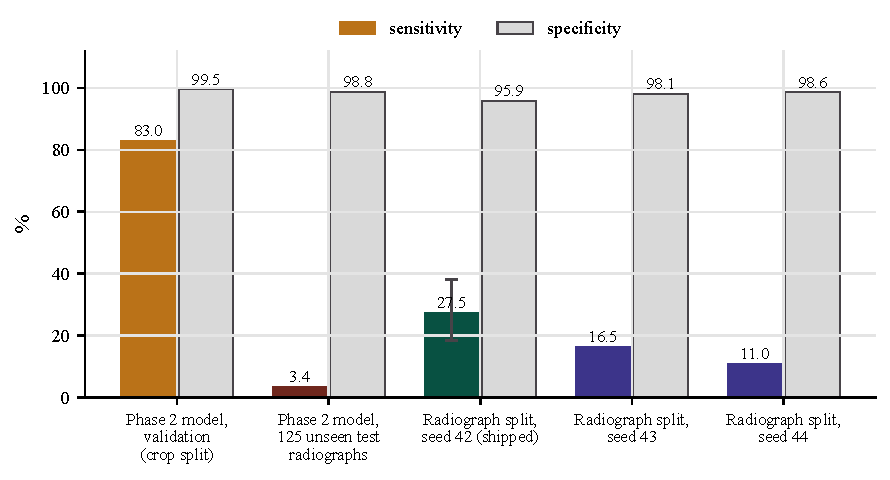
\includegraphics[width=0.94\textwidth]{figures/plots/P5_stage4_correction.pdf}
\caption[Stage 4a sensitivity and specificity]{Stage 4a sensitivity and specificity, from the Phase 2
validation figure to the radiograph-split retrain (error bar: 95\% interval of the shipped model).}
\label{fig:stage4}
\end{figure}

The severity head (macro-F1 0.294 [0.214, 0.385] against 0.334 for an image-blind position prior) stays
withheld, and no periodontal claim is made. The label itself is part of the explanation: the masks mark
apical lesions, sclerosis and cysts, so the collapse on external periodontitis annotations, where the
Phase 2 model found 2.4\% [2.0, 2.9] of the annotated teeth pooled over four Ningxia sites, is at least
partly a label mismatch rather than a failure to transfer. % {C042}

\section{Controls}
\label{sec:res-controls}

\textbf{Vision-language models without anatomy.} Shown no anatomy, the vision-language models return the
population prior. Qwen2.5-VL-7B answers ``26,~36'' to a blank grey image, to random noise and to a real
radiograph. Qwen2.5-VL-32B answers ``none'' to the blank image but answers noise with exactly the
constant's eight molars. One prompt was used and the decoding settings were not recorded, so this holds
for these models under this prompt. % {C019}

\textbf{Near-duplicate check.} A perceptual-hash search of the 164 scored DENTEX images against all 1,389
other DENTEX images found no further copy (Figure~\ref{fig:neardup}). As a positive control, all 86
MD5-identical images come out at distance 0 under both hashes, and all 86 were already excluded. No scored
image is at distance 0. The closest pHash pair is at 4 bits, with a dHash distance of 13. The 20
scored images with the nearest neighbours, inspected by eye, each differ from their neighbours in
restorations or missing teeth. The method finds copies of a radiograph, not a second radiograph of the
same patient. % {C060}

\begin{figure}[!htbp]
\centering
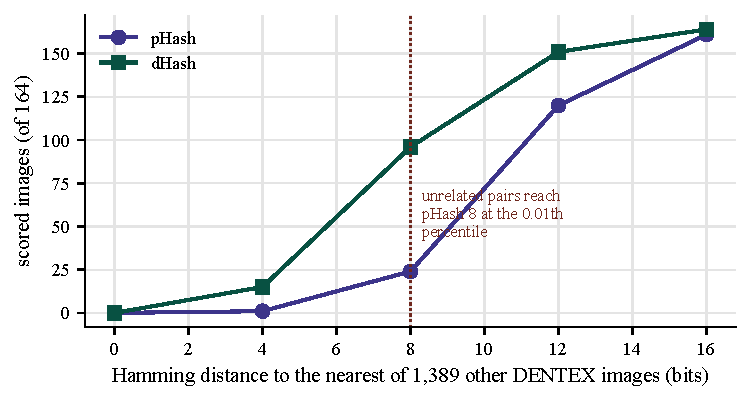
\includegraphics[width=0.78\textwidth]{figures/plots/P6_near_duplicates.pdf}
\caption[Near-duplicate check]{Scored DENTEX images whose nearest neighbour among the other DENTEX
images lies within a given Hamming distance, for pHash and dHash.}
\label{fig:neardup}
\end{figure}

\section{Runtime and Model Size}
\label{sec:res-runtime}

The whole pipeline runs at 1.70 seconds per image on the CPU of the team's macOS laptop, with no GPU
(1.45 seconds with the previous detector). The default configuration has 95.34\,M learnable parameters,
81.21\,M with the crop-classifier variant, and 72.99\,M for the caries path alone
(Figure~\ref{fig:params}). % {C001} {C003}

\begin{figure}[!htbp]
\centering
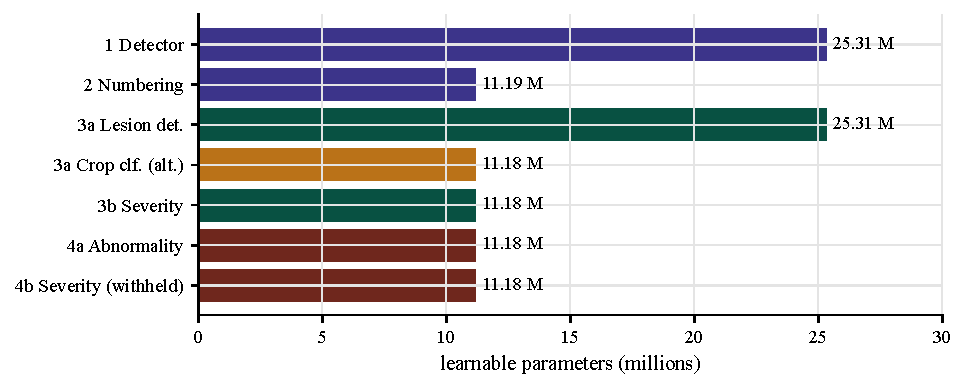
\includegraphics[width=0.86\textwidth]{figures/plots/P8_parameters.pdf}
\caption[Learnable parameters per stage]{Learnable parameters per stage, read from the saved weights
(batch-normalisation buffers excluded).}
\label{fig:params}
\end{figure}

\section{Discussion}
\label{sec:discussion}

The theory of Section~\ref{sec:method-constant} was formulated after the measurements, so
Table~\ref{tab:theory} is a consistency check, not a test of predictions made in advance. Five of its
implications hold, the last only at three of four sites; one of them is also expected under ordinary
domain shift and does not single out the theory. One is not supported: the prior inflates the
classifier's thresholded scores, but its ranking within a tooth type carries real image signal.

\begin{table}[!htbp]
\centering
\caption[What the theory implies, and what the measurements show]{What the theory implies, and what the
measurements show (a post-hoc consistency check).}
\label{tab:theory}
\small
\begin{tabularx}{\textwidth}{@{}L{4.2cm}YL{2.4cm}@{}}
\toprule
Implication & Evidence & Verdict\\
\midrule
Rule~\eqref{eq:rule} gives the best constant & reproduces the fitted eight molars; recall 0.600 equals the carious share at them & holds\\
The floor moves with the cohort & the constant's agreement is 0.494 to 0.709 across four sites & holds\\
A shortcut lifts healthy-tooth scores & healthy score 0.075 (incisors) to 0.478 (molars); 48.2\% of healthy molars flagged & holds\\
The shortcut carries the ranking & within-type AUC 0.745 [0.660, 0.842]; position-balanced AP $+0.043$ [$-0.033$, $+0.116$] & not supported\\
Development agreement does not transfer & classifier minus constant $+17.12$, $+0.89$ and $-22.42$ on the three cohorts & holds; not specific\\
Localising gives fewer, better flags & Ningxia $+9.28$ with 4.35 against 7.15 flags per image; DENTEX molar flags 46.3\% against 28.4\% carious & at 3 of 4 sites\\
\bottomrule
\end{tabularx}
\end{table}

\textbf{RQ1.} The same metric moves 40 points across cohorts and 31 across one cohort's sites, so a
favourable tooth-level figure on development data is weak evidence of perception.

\textbf{RQ2.} A detector that must place lesion boxes can express a positional prior only at a cost in
precision. It led the constant on the external sites with fewer flags, and on the development corpus its
flags were carious more often within each tooth type. Three facts qualify the lead:
\begin{itemize}
\item Ningxia informed the detector's adoption, so the lead measured there is optimistic.
\item The change of task is confounded with new training data.
\item The site-level interval includes zero; test1, where the constant is strongest, stays unexplained.
\end{itemize}

\textbf{RQ3.} Numbering, calibration and shuffle-controlled abstention are outputs a constant cannot
attempt, and they show confidence that ranks the system's own errors.

\textbf{What to report.} A tooth-level caries score should travel with an image-blind row fitted off the
test set, the identity factors of Table~\ref{tab:identity}, per-site external results with paired
intervals, and images of what the system does (Figures~\ref{fig:walkthrough}, \ref{fig:training}
and~\ref{fig:outcomes}). This complements the reporting checklists for medical-imaging and dental
AI~\cite{mongan2020claim,schwendicke2021checklist}. % {C090}

\section{Limitations}
\label{sec:limitations}

The authors' own limitations come first:
\begin{itemize}
\item DENTEX is in-domain for the tooth detector, which missed its Tufts guard (0.587 against 0.723).
  Only Ningxia is external to the lesion detector, it informed the adoption, and the random-effects
  interval includes zero. % {L001}
\item The theory treats codes independently and was checked on one corpus (78 and 164 images); the
  shortcut test rests on 34 radiographs; the lesion detector has no calibration curve. % {L002}
\item DENTEX caries labels were read from panoramic radiographs alone, which detect proximal caries less
  accurately than bitewings~\cite{akarslan2008comparison}. The expert lesions are therefore a subset of
  disease, and part of the molar prior may be a prior of what panoramic labels capture. % {L003}
\item Agreement has no negative class and the external cohorts have no healthy controls. Every model but
  Stage 4a is a single run, no clinician comparison was made, and the duplicate checks cannot find a
  patient's second radiograph. % {L004}
\item The Stage-4 label marks expert abnormalities, not periodontal bone loss; Stage 3b was validated
  only on 133 development crops. % {L005}
\end{itemize}

Additional caveats:
\begin{itemize}
\item The per-tooth-type comparison of flag precision was computed on DENTEX only. The saved Ningxia
  outputs hold per-image counts, so repeating it externally needs a re-run on the raw images.
\item The vision-language comparison used one prompt without recorded decoding settings.
\end{itemize}
